% Independent supplementary material.
\ifdefined\pdfminorversion\pdfminorversion=7\fi
\documentclass[10pt,twocolumn,letterpaper]{article}
% Shared formatting and notation for the paper and independent supplement.
\usepackage[review]{cvpr}
\usepackage{bm}
\usepackage{multirow}
\usepackage{tabularx}
\usepackage{makecell}
\usepackage{microtype}
\usepackage{placeins}
\usepackage{tikz}
\usetikzlibrary{arrows.meta,positioning,fit,calc,backgrounds,shapes.misc,decorations.pathreplacing}
\definecolor{cvprblue}{rgb}{0.21,0.49,0.74}
\usepackage{xr-hyper}
\usepackage[pagebackref,breaklinks,colorlinks,allcolors=cvprblue]{hyperref}
\def\confName{CVPR}
\def\confYear{2027}
\graphicspath{{figures/}}
\setlength{\tabcolsep}{3.4pt}
\renewcommand{\arraystretch}{1.05}
% cvpr.sty sets \hfuzz=30pt, which keeps overflows below 30pt out of the log. Report every
% overflow so that scripts/check_build.py sees it; this changes warnings only, not the layout.
\hfuzz=0.5pt

% Semantic colors shared by figures (docs/writing/cvpr_ai_writing_figure_guide.md).
\definecolor{obscol}{HTML}{0072B2}   % observation / history
\definecolor{predcol}{HTML}{E69F00}  % prediction / world
\definecolor{actcol}{HTML}{7B61A8}   % action
\definecolor{gtcol}{HTML}{4D4D4D}    % ground truth / neutral
\definecolor{failcol}{HTML}{D55E00}  % failure annotation
\definecolor{fillcolor}{HTML}{C2185B}% placeholders to be filled by the authors

% ======================================================================
% Author switches and configuration values for the v2 manuscript.
% Shared by main.tex, supplementary.tex, paper_full.tex, and manuscript_zh.tex.
% Guide: docs/writing/v2_author_guide.md (switch meanings, fill-in list).
% ======================================================================

% ---- Outcome switches -------------------------------------------------
% Predict / context resolution (Q2).
%   1 = role-allocated (expected): target SE(3) + coarse 3D context flow; finer grids
%       help only once the clearance falls to the coarse flow's path error.
%   2 = metric 3D is what matters: context resolution has no measurable effect down to
%       the tightest clearance swept (which stays above the coarse flow's error).
%   3 = finer context flow helps at the tight clearances of the tasks; the final model
%       uses the coarsest grid that preserved success (set \cfgContextSide below).
\newcommand{\QtwoCase}{1}

% Act / world-action coupling (Q3). World = object query + scene queries (deterministic regression).
%   1 = hidden-state access: action tokens read the world queries' keys/values at every layer (R2);
%       the world does not read actions (Q3-INFO0 program R2).
%   2 = explicit geometry: the decoded target SE(3) trajectory and scene flow are re-encoded as
%       geometric condition tokens for the action, end to end, no teacher forcing (R5-Y).
%   3 = world as training signal only; action-only deployment (R1, no test-time imagination).
% Set to 3 on 2026-10-20 from Research Q3-INFO0 (three seeds each, 1,400 development scenes):
% R2, R3, R4 and R5-Y gave no stable gain over R1 (R1 63.60%, R2 62.52%, R3 64.21%, R4 63.00%,
% R5-Y 63.95%), and disabling the world objectives (R0, 60.45%) was lower on average.
% Re-check on held-out scenes before submission; author guide section 2 lists what to re-check.
\newcommand{\QthreeCase}{3}

% Backbone parameterization.
%   1 = shared attention projections, stream-specific feed-forward networks.
%   2 = separate world and action parameter groups (attention, AdaLN, FFN); condition
%       tokens are processed by the world group, so world losses still shape what the
%       action reads even when no cross-stream edge is open (QthreeCase = 3).
% 1 per Research BACKBONE0 (2026-10-20): D 66.76% vs. E 62.86%, three seeds, matched parameters.
\newcommand{\BackboneCase}{1}

% ---- Names -------------------------------------------------------------
\newcommand{\ours}{SE(3)-WAM\xspace}
\newcommand{\bench}{Dynamic-14\xspace}

% ---- Configuration of the final model (confirm before submission) ------
\newcommand{\cfgVisualEncoder}{MAE ViT-B/16}   % frozen observation encoder (SCALE0: frozen MAE-B selected)
\newcommand{\cfgLayers}{4}
\newcommand{\cfgWidth}{768}
\newcommand{\cfgHeads}{8}
\newcommand{\cfgBackboneParams}{47.3M}    % trainable backbone parameters (both parameterizations, matched)
\newcommand{\cfgTrainableParams}{62.2M}  % all trainable parameters, frozen MAE encoder and DINO teacher excluded (BACKBONE0 core count)
\newcommand{\cfgHistoryLen}{8}          % history samples
\newcommand{\cfgHistorySpan}{350\,ms}   % history span
\newcommand{\cfgHorizons}{8}            % number of prediction horizons
\newcommand{\cfgHorizonStep}{50\,ms}
\newcommand{\cfgMaxHorizon}{400\,ms}
\newcommand{\cfgPatches}{196}           % current-image patch tokens
% Context-flow grid of the final model: set the side only; the grid and the point count follow.
% With \QtwoCase=3, set it to the grid the clearance study selected (e.g. 28).
\newcommand{\cfgContextSide}{14}
\newcommand{\cfgContextGrid}{$\cfgContextSide\times\cfgContextSide$}
\newcommand{\cfgContextPoints}{\number\numexpr\cfgContextSide*\cfgContextSide\relax}
\newcommand{\cfgChunk}{8}               % commands per action chunk
\newcommand{\cfgEuler}{5}               % Euler steps per generated stream
\newcommand{\cfgControlRate}{20\,Hz}
\newcommand{\cfgLatencyMax}{250\,ms}    % training latencies are sampled from U[0, this]
\newcommand{\cfgReplan}{100\,ms}        % executor's replanning interval
\newcommand{\cfgRobot}{a seven-DoF Franka arm with a parallel-jaw gripper and a calibrated RGB-D camera}
\newcommand{\cfgRobotZh}{配备平行夹爪与标定 RGB-D 相机的七自由度 Franka 机械臂}
\newcommand{\cfgGPU}{RTX~5090}       % deployment GPU (32 GB); every method's latency is measured on it
\newcommand{\cfgTrainHardware}{eight RTX PRO 6000 GPUs}  % Research BACKBONE0/Q3-INFO0 training runs (world8)
\newcommand{\cfgTrainHours}{7.7}       % hours per training seed on \cfgTrainHardware (Q3-INFO0 timing_reference: 7.60-7.73 h)
\newcommand{\cfgTrainHardwareZh}{8 块 RTX PRO 6000 GPU}


% ---- Placeholders ------------------------------------------------------
% \fillin{...}: a value or phrase the authors must supply (colored in the PDF).
% \resultplaceholder: a pending table cell. scripts/check_build.py counts both.
% The dash is centred in the width of a typical entry (default "00.0"), so table widths, and
% hence the page layout, already match the filled-in paper. Cells with another format pass
% their own template, e.g. \resultplaceholder[{+00.0 [00.0, 00.0]}].
\newcommand{\fillin}[1]{\textcolor{fillcolor}{[#1]}}
\newcommand{\resultplaceholder}[1][00.0]{\textcolor{fillcolor}{%
  \begingroup\setbox0=\hbox{#1}\hbox to \wd0{\hfil\textemdash\hfil}\endgroup}}
% \figplaceholder[height]{width}{title}{specification}
\newcommand{\figplaceholder}[4][1.6in]{%
  \fcolorbox{fillcolor!70}{fillcolor!3}{%
  \begin{minipage}[c][#1][c]{\dimexpr#2-2\fboxsep-2\fboxrule\relax}%
  \centering{\small\sffamily\bfseries\color{fillcolor}Figure placeholder: #3}\par\vspace{3pt}%
  {\scriptsize\sffamily\raggedright #4\par}%
  \end{minipage}}}

% ---- Outcome switches (values in paper_config.tex) ----------------------
% \Qtwo{n}{text} prints text only when \QtwoCase = n; likewise \Qthree and \Bbone.
\newcommand{\Qtwo}[2]{\ifnum\QtwoCase=#1\relax#2\fi}
\newcommand{\Qthree}[2]{\ifnum\QthreeCase=#1\relax#2\fi}
\newcommand{\Bbone}[2]{\ifnum\BackboneCase=#1\relax#2\fi}
\newcommand{\QtwoSel}[3]{\ifcase\QtwoCase\relax\or#1\or#2\or#3\fi}
\newcommand{\QthreeSel}[3]{\ifcase\QthreeCase\relax\or#1\or#2\or#3\fi}
\newcommand{\BboneSel}[2]{\ifcase\BackboneCase\relax\or#1\or#2\fi}
% Marks the configuration selected for the final model in design tables.
\newcommand{\sel}{$^\star$}
% Marks the context-flow grid of the final model (\cfgContextSide in paper_config.tex).
\newcommand{\gridsel}[1]{\ifnum\cfgContextSide=#1\relax\sel\fi}

% Cross-document references. The full edition resolves every label directly;
% main.tex and supplementary.tex redefine these to read each other's .aux file,
% so scripts/build.ps1 compiles the supplement before the paper.
\newcommand{\appref}[1]{\ref{#1}}
\newcommand{\mainref}[1]{\ref{#1}}

% ---- Notation -----------------------------------------------------------
\newcommand{\se}{\ensuremath{\mathrm{SE}(3)}\xspace}
\newcommand{\so}{\ensuremath{\mathrm{SO}(3)}\xspace}
\newcommand{\R}{\ensuremath{\mathbb{R}}\xspace}
\newcommand{\Exp}{\operatorname{Exp}}
\newcommand{\Log}{\operatorname{Log}}
\newcommand{\vect}[1]{\mathbf{#1}}
\newcommand{\tapp}{\tau^{\mathrm a}}
\newcommand{\takeaway}[1]{\par\smallskip\noindent\textbf{Takeaway.} \emph{#1}\par\smallskip}
% Shared tables keep one set of numerical cells for both reading editions.
\newcommand{\tablelang}[2]{#1}
\usepackage{amssymb}
\providecommand{\cmark}{\ensuremath{\checkmark}}

\hypersetup{pdfauthor={Anonymous Authors},pdftitle={SE(3)-WAM: Supplementary Material}}
\title{SE(3)-WAM: What Should a Robot Remember and Predict\\for Dynamic Manipulation?\\Supplementary Material}
\author{Anonymous Authors}
\begin{document}
\maketitle
\renewcommand{\thetable}{S\arabic{table}}
\renewcommand{\thefigure}{S\arabic{figure}}
\renewcommand{\theequation}{S\arabic{equation}}
This supplement expands the completed simulation studies and specifies the
unfinished experiments. Measured values preserve each study's information
track, endpoint, and evaluation partition. Red fields identify results or
interfaces still to be supplied. The reading map connects these details to
the separate main paper.
\begin{table}[h]
\centering\small
\begin{tabularx}{\columnwidth}{@{}lXl@{}}
\toprule
Appendix & Contents & Main \\
\midrule
A & Tasks, data, information, scoring & Sec.~3 \\
B & Reference implementation and budgets & Secs.~4--5 \\
C & Current-pose history comparison & Sec.~5.4 \\
D & Fifteen future objectives and combinations & Secs.~5.2--5.3 \\
E & Backbone, information flow, cross-checks & Secs.~4.4, 5.6 \\
F & Pretraining, deployment, external tests & Sec.~5.6 \\
G & Failures and qualitative evidence & Sec.~5.5 \\
\bottomrule
\end{tabularx}
\end{table}
\appendix
\section{Tasks, Data, and Evaluation}
\label{app:protocol}

\subsection{The Reported Fourteen-Task Suite}
The completed studies use the migrated DB0 v0.6 demonstration pool and its
fourteen-task evaluation suite. Table~\ref{tab:tasks} lists the task identifiers
used in the result arrays. The task-balanced
score includes every task, including zero-success conditions.

\begin{table*}[!t]
\centering\fontsize{9}{11}\selectfont
\setlength{\tabcolsep}{4pt}
\renewcommand{\arraystretch}{1.13}
\caption{Native success conditions in the reported fourteen-task suite.
Thresholds come from the evaluator source and task configurations bound to the
accepted FUTURE0, BASE2, and HISTORY1 packages. A task must pass its preceding
stages and avoid terminal failures. All tasks run at 20\,Hz with a 2\,ms physics
step; durations below refer to physical time. COM denotes center of mass.}
\label{tab:tasks}
\begin{tabularx}{\textwidth}{@{}p{0.19\textwidth}Xp{0.07\textwidth}@{}}
\toprule
Task & Ordered success conditions & Limit \\
\midrule
grasp;\newline t1\_belt, t1\_xyz,\newline t1\_so3, t1\_occ
& Approach within 0.10\,m; bilateral fingerpad contact for 0.05\,s; collision-geometry
bottom at least 0.05\,m above support; retain contact and clearance for 0.50\,s.
T1 adds conveyor drive, translation, rotation, or a physical occluder.
SO3 has no additional success-angle threshold; unsafe occluder contact terminates OCC.
& 160 steps\newline 8\,s \\
t2\_trans
& Approach within 0.10\,m. Entire object collision geometry inside the receptacle:
planar clearance and floor gap both $\geq-0.002$\,m, top no higher than the opening.
Release requires an opening command $<-0.5$ and no fingerpad contact.
Relative linear/angular speeds $\leq0.08$\,m/s and $0.8$\,rad/s for 0.10\,s,
followed by a 0.50\,s stable dwell.
& 200\newline 10\,s \\
t2\_se3
& Approach within 0.05\,m and 0.12\,rad. Full T-shaped containment:
planar clearance $\geq0.002$\,m, floor gap in $[-0.002,0.002]$\,m,
tilt $\leq0.05$\,rad, top below opening.
After release, relative speeds $\leq0.02$\,m/s and $0.04$\,rad/s
for 0.10\,s, then a 0.50\,s dwell. The 0.12\,rad gate applies to approach.
& 200\newline 10\,s \\
t3\_phase
& Start with the native pre-grasp. Phase alignment: distance $\leq0.090$\,m and
loop-direction error $\leq0.20$\,rad. Enter within 0.030\,m at progress $\leq0.15$;
reach historical maximum progress $\geq0.60$, then $\geq0.85$ and endpoint
distance $\leq0.055$\,m.
& 420\newline 21\,s \\
t3\_full
& Acquire the wand with bilateral contact for 0.05\,s, then complete the phase
stages above. In a later sample, retain current progress $\geq0.85$ and move
at least 0.045\,m from both path and endpoint. Finally open ($<-0.5$)
with no fingerpad contact. Releasing before exit fails.
& 640\newline 32\,s \\
t4\_sphere
& Approach within 0.10\,m; first qualifying contact after ramp exit; any tray contact before success
fails. Bilateral hold for nominal 25\,ms (12 physics samples, 24\,ms).
Raise COM by 0.05\,m from its height when the bilateral-hold criterion is first met, and retain
contact and height for 0.50\,s.
& 120\newline 6\,s \\
t4\_sphere\_tabletop;\newline t4\_slider
& Approach within 0.10\,m; contact after ramp exit, while supported, in the capture region, and moving
at planar speed $\geq0.08$\,m/s. Bilateral hold for 0.05\,s, COM lift
$\geq0.05$\,m from the first attainment of that hold criterion, then contact and height for 0.50\,s.
& 120\newline 6\,s \\
t4\_can
& Same supported-capture sequence. Before first fingerpad contact, a can-axis
absolute dot product with vertical $>0.45$ fails as unstable tipping.
The configuration does not require a transverse closing axis.
& 120\newline 6\,s \\
t5\_replan
& Exactly one selected-side impact group completes before robot contact.
At 30\,ms after the physical impact-end timestamp, branch-signed lateral speed $\geq0.035$\,m/s and yaw rate
$\geq0.35$\,rad/s. Approach within 0.10\,m; bilateral hold with grasp-axis
error $\leq18^\circ$ for 0.05\,s; COM lift $\geq0.05$\,m from the first
attainment of that hold criterion and stable hold
for 0.50\,s. Impact-group lag is 12\,ms and maximum contact is 0.10\,s.
& 120\newline 6\,s \\
\bottomrule
\end{tabularx}
\end{table*}


\begin{figure*}[t]
\centering
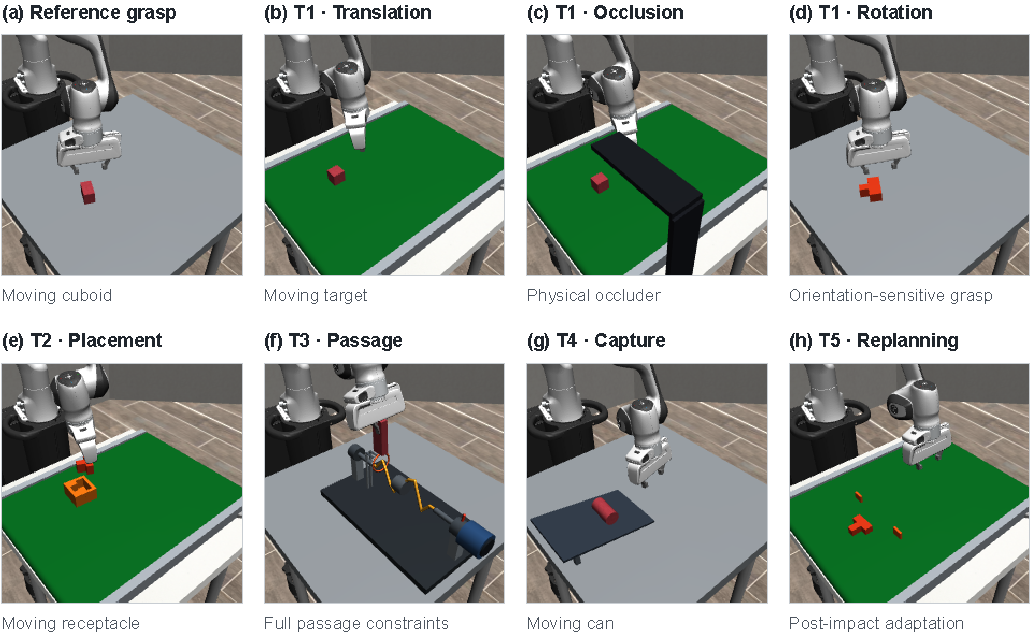
\includegraphics[width=\textwidth]{benchmark_task_examples.pdf}
\caption{Recorded benchmark observations. Eight examples cover reference
grasping; T1 translation, physical occlusion, and orientation-sensitive grasping;
T2 moving-receptacle placement; T3 constrained passage; T4 capture; and
T5 post-impact adaptation. For each displayed task, the lowest state index
in the accepted DEV84 manifest supplies the final observed, uncropped
$224\times224$ agentview RGB. Labels identify task conditions; the snapshots
illustrate appearance and geometry, while task outcomes are reported separately.
Table~\ref{tab:tasks} lists all fourteen tasks.}
\label{fig:benchmark_tasks}
\end{figure*}

The common training pool has 11,200 episodes, 800 per task. The internal
representation screen uses 350 validation episodes; adapted systems retain
their own validation settings (including 1,400 for DreamVLA/OpenWAM).
The future screen samples 160,416 chunks per epoch. Stored episode
count and effective chunk exposure measure different aspects of training.
Later fresh-data production retains its own data identity and does not
retroactively change the source of these results. Motion-only P0 prediction
has no corresponding action-learning score in the fourteen-task table.

Success is read from the native task evaluator after its ordered physical
requirements (Table~\ref{tab:tasks}). The accepted FUTURE0, BASE2, and HISTORY1
packages reference the same archived evaluator source, task configurations,
and fourteen-suite scenario manifest. We recover the definitions from that
archive. Success is checked at each 2\,ms physics step. Interrupted continuous
conditions reset their counters. For T2, the sample completing the low-relative-motion
counter also starts the stable-dwell counter; the two durations should not
be added as an exact 0.600\,s requirement.

\paragraph{Terminal events.}
The native result mapping groups events into five categories:
\emph{invalid} (invalid state);
\emph{boundary} (workspace or downstream exit, drop, expired goal window);
\emph{safety} (unsafe contact, excessive rim impulse, wire contact, stage block,
release impulse, early robot contact, tray or gripper--support contact,
striker trap);
\emph{task violation} (blocked driver, release outside the goal, path deviation
or backtracking, premature release, stopping/deflecting without capture,
unstable tipping, missing/extra impact, wrong striker contact, or insufficient
outgoing motion change);
and \emph{timeout}. These categories describe evaluator outcomes.

There is no global priority among categories. Each family selects the first
terminal event in its physics-step evaluation order and preserves that result.
Grasp checks invalid state, workspace exit, downstream exit, and drop before
success, then timeout. T1 inserts unsafe occluder contact after invalid state.
T2 checks invalid state, rim impulse $>0.10$\,N\,s, drop, goal-window expiry,
and release outside the goal before success and timeout.
T3 checks invalid state, stage block, drop, workspace exit, wire contact,
premature release, path deviation, and backtracking before success and timeout.
Wire failure uses impulse $>0.020$\,N\,s or penetration $>0.004$\,m for more
than two consecutive steps; path deviation is $>0.030$\,m for 0.050\,s,
and backtracking exceeds 0.05 relative to maximum progress.

T4 checks invalid state, release impulse $>0.002$\,N\,s, unsafe ramp contact,
unsupported tray contact, can tipping, early-contact/boundary branches,
and invalid supported capture before success and timeout.
A target that has exited the ramp, remains in contact with the downstream
support, and has no fingerpad contact at speed $\leq0.03$\,m/s for 0.25\,s
fails as stopping/deflecting only.
T5 checks invalid state, unsafe contact, early robot contact, wrong striker,
extra impact/striker trap, insufficient outgoing change, and boundary events
before success. At the horizon, zero completed impacts yields missing selected
impact; otherwise the result is timeout.

\subsection{Scenario Sampling and Replay}
\begin{table*}[!t]
\centering\fontsize{9}{11}\selectfont
\setlength{\tabcolsep}{4pt}
\renewcommand{\arraystretch}{1.12}
\caption{Historical validation proposal ranges. Length, linear velocity, angle,
and angular velocity use m, m/s, rad, and rad/s unless marked otherwise.
Positions are in world coordinates except the stated ramp-local offsets.
Continuous intervals are uniform proposals; discrete choices are equiprobable
before feasibility checks. Evaluation replays the stored accepted scenarios,
whose distribution need not remain uniform. Harmonic centers are not initial positions.}
\label{tab:task_sampling}
\begin{tabularx}{\textwidth}{@{}p{0.18\textwidth}p{0.34\textwidth}X@{}}
\toprule
Task & Initial-state proposal & Motion or event parameters \\
\midrule
grasp & Harmonic center $c_x\in[-.08,.08]$, $c_y\in[-.26,-.19]$, $z=.822$;
yaw $[-1.1,1.1]$.
& $v_y\in[.025,.125]$, $A_x\in[.015,.035]$, $f_x\in[.3,.7]$\,Hz;
$\omega_z\in[-1.2,1.2]$. \\
t1\_belt & Target $x\in[-.08,.08]$, $y\in[-.26,-.18]$, $z=.822$;
identity orientation, zero initial twist.
& Belt $v_y\in[.04,.10]$. \\
t1\_occ & Same target proposal as Belt; canopy at $(.322,-.29,1.20)$.
& Same belt range; clearance parameter .20; physical occlusion. \\
t1\_xyz & Harmonic center $c_x\in[-.025,.025]$, $c_y\in[-.24,-.20]$, $z=.818$;
yaw $[-.35,.35]$.
& $v_y\in[.04,.09]$, $A_x\in[0,.03]$, $f_x\in[.25,.65]$\,Hz; $\omega_z=0$. \\
t1\_so3 & Same as XYZ.
& Same translation; $\omega_z\in[-1.2,-.4]\cup[.4,1.2]$, equal sign probabilities. \\
t2\_trans & Goal $x\in[-.13,-.08]$, $y\in[-.18,-.12]$, $z=.825$; fixed orientation.
& Goal $v_y\in[.03,.06]$; no rotation. \\
t2\_se3 & Same goal $x,y$ range, $z=.804$; yaw $[-.3,.3]$.
& Goal $v_y\in[.03,.06]$;
$\omega_z\in[-.25,-.08]\cup[.08,.25]$, equal sign probabilities. \\
t3\_phase & Wand $x,y\in[-.03,.03]$, $z=.870$, yaw $[0,2\pi]$;
wire phase $[-.25,.35]$.
& Wire center $(.10,-.02,.94)$; world-X rotation
$\omega_x=-\{2.5,3,\ldots,7.5\}^{\circ}$/s (11 equal-probability values). \\
t3\_full & Wand at $(-.05,-.02,1.04)$ with identity orientation;
same wire phase range.
& Same wire rotation; cradle and release requirement enabled. \\
t4\_sphere & Ramp-local offsets: lateral $[-.015,.015]$, longitudinal/normal
$(-.145,.030)$; lip $(.06,-.02,1.10)$.
& Gravity-driven from rest; gate release at tick 0; slope $[5,15]^\circ$;
target/ramp sliding friction $[.7,.9]$; unsupported capture. \\
t4\_sphere\_tabletop & Lateral $[-.015,.015]$, longitudinal/normal
$(-.124,.034)$; lip $(0,-.06,.808)$.
& Same slope and release; target/ramp friction $[.7,.9]$, table friction .35. \\
t4\_slider & Lateral $[-.015,.015]$, longitudinal/normal $(-.129,.024)$;
supported ramp.
& Same slope and release; target/ramp friction $[.025,.045]$,
table friction $[.012,.018]$. \\
t4\_can & Lateral $[-.010,.010]$, ramp-axis yaw $[-4,4]^\circ$;
longitudinal position follows gate geometry and oriented can extent.
& Same slope and release; target/ramp friction $[.25,.45]$,
table friction $[.09,.15]$. \\
t5\_replan & $x\in[-.005,.005]$, $y=-.29$, $z=.812$;
yaw $[-.08,.08]$; zero initial twist.
& Belt $v_y\in[.12,.14]$; equal-probability left/right striker triggered at
$y=-.13$; stroke .098, pulse .35\,s, actuator scale $[1,1.1]$,
force cap 4\,N; command delay 50\,ms. \\
\bottomrule
\end{tabularx}
\end{table*}

The historical E7/agentview recipes specify proposal ranges
(Table~\ref{tab:task_sampling}). Continuous min--max fields use uniform draws
from NumPy PCG64; discrete choices are equiprobable before physical-feasibility
checks. Evaluation loads each accepted scene's complete stored ScenarioSpec
and does not resample its parameters.
For harmonic translation,
\[
p(t)=c+(0,v_y,0)t+(A_x\sin(2\pi f_xt+\phi),0,0),
\]
where $\phi\sim U[-\pi,\pi]$. Thus $c$ differs from the initial position by
the phase-dependent offset. T4 targets start at zero linear/angular velocity
and evolve under free dynamics; no constant target speed is prescribed.
Their slope is continuously sampled from $[5,15]^\circ$.
Ramp-local offsets use the ramp center as origin and lateral, downhill,
and normal axes: $p_{\rm world}=c_{\rm ramp}+R_x(-\alpha)p_{\rm offset}$.
The center is derived from the exit lip and ramp half-size; offsets are
not added directly to the lip.
T2-SE3 training uses $\omega_z\sim U[-.25,.25]$; validation excludes
$(-.08,.08)$. The other thirteen tasks share train/validation proposal recipes.

Occlusion acceptance requires at least eight initially visible frames with
visible fraction $\geq.95$, ten to sixty fully occluded frames
(fraction $\leq.05$, lasting 0.5--3.0\,s), and at least three reappearance
frames with fraction $\geq.8$. These are acceptance criteria, not independent
sampling variables. For example, the accepted OCC scenes have belt speeds
0.059588--0.099852\,m/s within the wider proposal interval.
Accepted source seeds can have gaps; a consecutive seed range does not
reconstruct the scene set.

All 1,400 stored scenarios share the robot joint initialization
\[
\begin{aligned}
q_0={}&[0,\ .19634954,\ 0,\ -2.61799388,\\
      &0,\ 2.94159265,\ .78539816]\ {\rm rad},
\end{aligned}
\]
and finger positions $(.020833,-.020833)$\,m.
T4 additionally stores a temporary preparation-target pose with
$x,y\sim U[-.03,.03]$ and yaw $U[0,2\pi]$, distinct from the release state.

The evaluator source stores recipes in \path{configs/scenarios/}
and task bindings in \path{configs/tasks/}; the generation entry point is
\path{se3_wam_benchmark/cli/generate_scenarios.py}.
The evaluation payload contains the concrete
\path{evaluation_reference/scenes/validation.jsonl} and fourteen
\path{evaluation_reference/scenes/suites/sr_<task>.yaml} files.
Each suite uses one repeat and filters the shared manifest by task.
These files, with the stored scenario IDs and source seeds, define the
replay set used for the paired comparisons.

The accompanying local material package at
\path{results/replay_materials/} contains the archived evaluator, task and
sampling configurations, all accepted scenarios, and both ordered selections.
Portable copies change only execution paths; originals are retained.
The archived manifest parser reads all 1,400 scenarios without changing their
scientific fields, and the task/configuration loaders read all fourteen
definitions. The supplied checker also verifies disjoint partitions, identities,
seeds, and asset references. These checks parse the materials; physics and
policy replay require the additional runtime and model assets listed in the
package instructions.

\subsection{Partitions and Statistical Interpretation}
The 140-scene development set has ten scenes per task. Its disjoint complement
has ninety per task, totaling 1,260. The future screen reports the two
partitions separately. The system-reference study also keeps them separate.
The combination screen explicitly selects on all 1,400 scenes while retaining
both component counts. Thus its selection score includes development data,
and the 1,260 complement is now part of the project's development evidence.
Neither membership disjointness nor a different rollout seed makes it a final
blind test.

The future study uses each condition's own fourth-epoch endpoint and one
training seed. Across arms, the scene, source seed, and inference seed are
paired. There are 18,900 accepted outcomes, 1,260 per arm; missing scenes and
infrastructure-error exclusions are zero. Inference seeds span
20261058--20262317 for the designated selection indices. Matching an inference
seed specifies rollout randomness but does not imply that unlike training
graphs consumed identical random-number sequences.

For two policies on the same scenes, let $b$ count candidate successes/reference
failures and $c$ candidate failures/reference successes. Then
\begin{equation}
 \Delta\mathrm{SR}=100(b-c)/1260
\end{equation}
in percentage points. The report uses the exact two-sided McNemar test on
discordant pairs. Fourteen comparisons to P00 and thirteen to P03 form the
twenty-seven-comparison family; adjusted values use
$\min(1,27p)$. The 378 task-level comparisons remain exploratory.

We additionally compute 95\% pointwise percentile intervals by resampling paired
scenes within each task. For every replicate, each task retains ninety pairs
(one hundred in the combination study), and the fourteen task differences are
averaged with equal weights. Sampling a multinomial from each task's four
paired outcome counts is equivalent to resampling its binary scene pairs.
We use 100,000 replicates and the 2.5th/97.5th percentiles with linear interpolation.
The generator is NumPy 2.3.5 PCG64; seeds are 20261017 plus the zero-based
lexicographic comparison index for the twenty-seven future contrasts,
and 20261017/20261018 for I versus F/E. The post-hoc I--E analysis excluding
phase passage retains thirteen tasks with seed 20261019.
Tasks are processed in lexicographic order.
These intervals condition on the trained checkpoints and fixed task mixture;
they do not include training-seed variation or candidate-selection uncertainty.
They are not simultaneous intervals; the corrected McNemar family above
remains the basis for the overall future-screen comparisons.

\subsection{Inputs and Time}
The completed future screen uses one current fixed-camera RGB view, exact
depth/camera geometry, robot-state history, and privileged object information.
A simulator field stored beside an image is not automatically a deployable
sensor observation. Future target states and label-validity masks supervise
their respective branches and are excluded from the action condition.
A current-object-pose oracle and a future oracle are distinct information
conditions.

Physical high-level steps are separated by 50\,ms. All one hundred T5 scenarios
use a one-step command delay (50\,ms); the other thirteen tasks use zero.
The native action queue returns a zero command until the delay elapses,
then applies the oldest queued command. Forecast labels cover
50--400\,ms relative to the source observation. Synchronous evaluation pauses
the environment for policy computation, so it cannot measure the consequence
of wall-clock observation age. Later fixed-delay and real-delay evaluations
must retain their own time traces and report whether physics continues while
the policy computes. Future labels follow the demonstration's recorded
geometry under its executed actions. The current validity masks check
geometric support, projection, and visibility. They do not establish that the
same post-contact future remains valid for an alternative candidate action.
Action-consistent label support is \placeholder{pending for online generation}.

\section{Reference Implementation and Budgets}
\label{app:implementation}

\subsection{Actual Representation-Screen Configuration}
The reference D model uses \texttt{se3wam\_v2/split\_ffn}, four transformer
layers, width 768, eight attention heads, and factorized attention.
DINOv3 ViT-L/16 is frozen \cite{dinov3}. A $224\times224$ agent-view image
produces 196 current visual tokens. H0V has zero visual-history query tokens.
The information track also supplies exact depth and camera geometry.
Robot input retains eight EEF7 states at 20\,Hz. Eight object tokens encode
current GT pose and seven motion intervals using 25 numeric statistics and
pose/interval/acceleration validity flags.

The object statistics include position, rotation vector, interval translation
and relative rotation, elapsed time, linear/angular velocity, and
linear/angular acceleration. Their source is simulator truth in this track.
The current-pose history track removes historical object poses and all derived
interval kinematics while preserving the current pose and robot history.
This is a different information condition, not a different name for the same
input.

D shares attention QKV/output projections and splits feed-forward networks
by world/meta, flow, and action stream. Scene tokens access scene tokens;
meta tokens access scene and meta; flow accesses scene and flow; action
accesses meta and action. Consequently, flow supervision can change shared
weights without an online flow-to-action path. The deterministic pose head
pools sixteen final meta tokens. Calling the model world--action does not
change these actual access relations.

\subsection{Coordinates, Losses, and Generation}
Target future translation is cumulative displacement in the fixed metric
frame. Rotation is the left-relative vector
$\phi_h=\Log(R_{t+\delta_h}R_t^\top)^\vee$.
For valid targets $\mathcal V$, the pose loss is
\begin{equation}
\begin{split}
 \mathcal L_{\rm pose}=\frac{1}{|\mathcal V|}\sum_{h\in\mathcal V}
 \big[&\|\hat d_h-d_h\|_2^2\\
 &+0.1\,d_{\mathrm{SO}(3)}(\hat R_{t+\delta_h},R_{t+\delta_h})^2\big].
\end{split}
\end{equation}
The external weight multiplying this loss is separate from the internal
rotation coefficient. A full twist exponential would couple translation
to rotation through its Jacobian and is not the implemented parameterization.
The reported configuration does not include the former draft's heteroscedastic
pose likelihood, uncertainty bridge, symmetry-minimized loss, or pose--flow
consistency objective.

The action has eight E7 steps: base-frame translation increment, left-relative
rotation vector, and gripper command. Translation and rotation training bounds
are 0.05\,m and 0.5\,rad per axis. The inherited evaluation translation
limit is 0.10\,m per axis. Action flow matching uses a unit Gaussian in
training-normalized action coordinates. Scene flow uses a metric Gaussian
source with standard deviation 0.02\,m. Deterministic auxiliary readouts,
including pose, do not consume flow-matching source noise and time.

Only the action generator runs during Q2 deployment, using five Euler steps.
Conditioning caching is on; temporal/velocity caching is off.
Each replan executes one command. Trainable initialization is fresh
for seed 0 rather than inherited from a trained common-reference checkpoint.
Global batch is 16. Four epochs produce 40,104 updates and 641,664 chunks.
P00, P02, and P05 finish with an eight-device topology; other arms finish
with sixteen. Some retained runs have recorded topology transitions.
These histories preserve the declared exposure and endpoint but do not
establish bitwise equivalence across topology.

\subsection{Alternative Target Definitions}
P04 uses a frozen Wan video VAE target. Nine RGB input frames produce three
temporal latents in the target construction; this is not eight independent
future latent frames. P05 uses dense cumulative 2-D displacement. P06 uses
real codec block motion vectors with reference, direction, and validity.
P07 uses sparse scene tracks and visibility, P08 pooled object DINO features,
and P09 target tracks and visibility. P08/P09 adapt mechanisms rather than
reproduce an entire published model.

Aalpha adds motion-magnitude MSE with weight 0.5 while preserving P03's
Alpha-head initialization. P12, P13, and P14 add future depth, spatial DINO,
and dynamic-region RGB supervision. P15 combines these three at their
individual weights. A non-existent head has an inapplicable readout,
not a zero error. The combination cannot identify every pairwise interaction.
Raw total losses across these objectives are not commensurate.

\subsection{System-Reference Training}
% Transcribed from Research BASE1 and the FUTURE0/BASE2 seed-0 reports.
\begin{table*}[t]
\centering\small
\caption{\tablelang{Training exposure and development counts for all system-reference
endpoints. Batch is global; all endpoints use training seed 0. Initialization
and execution are part of each adapted system, not matched factors.
The two DreamVLA endpoints are independent training schedules.
The 1,260-scene counts appear in the main system table.}{所有系统参照端点的训练量和开发集成功数。Batch 为全局批大小；所有端点的训练 seed 均为 0。初始化与执行方式属于各适配系统自身的设置，并非匹配因素。两个 DreamVLA 端点采用独立训练计划。1,260 场补集的计数见正文系统比较表。}}
\label{tab:system_budgets}
\begin{tabularx}{\textwidth}{@{}lrrrX@{}}
\toprule
\tablelang{System}{系统} & \tablelang{Updates}{更新次数} & \tablelang{Batch}{批大小} & \tablelang{Success /140}{成功数 /140} & \tablelang{Execution / initialization note}{执行与初始化说明} \\
\midrule
ACT & 50,000 & 32 & 50 & \tablelang{Scratch; temporal aggregation}{从头训练；时间聚合} \\
Diffusion Policy & 50,000 & 32 & 54 & \tablelang{Scratch; execute 8 actions}{从头训练；执行 8 个动作} \\
$\pi_{0.5}$ & 30,000 & 256 & 89 & \tablelang{\texttt{pi05\_base}; execute 10}{\texttt{pi05\_base}；执行 10 个动作} \\
DynamicVLA & 50,000 & 44 & 24 & \tablelang{Official DOM checkpoint; native continuous pipeline}{官方 DOM 检查点；原生连续流水线} \\
OpenWAM-Alpha & 34,490 & 192 & 76 & \tablelang{Official Alpha foundation; execute 32}{官方 Alpha 基础模型；执行 32 个动作} \\
DynamicWAM & 40,000 & 128 & 72 & \tablelang{Official full initialization; execute 16}{官方完整初始化；执行 16 个动作} \\
\tablelang{DreamVLA: 20 epochs}{DreamVLA：20 轮} & 48,220 & 512 & 112 & \tablelang{Independent schedule; aggregate forecasts, execute 1}{独立训练计划；聚合预测，执行 1 个动作} \\
\hspace{1em}\tablelang{40 epochs}{40 轮} & 96,440 & 512 & 114 & \tablelang{Independent longer schedule}{独立的更长训练计划} \\
\midrule
\tablelang{Study P00}{本研究 P00} & 40,104 & 16 & 88 & \tablelang{Fresh task network; frozen DINO-L; execute 1}{新训任务网络；冻结 DINO-L；执行 1 个动作} \\
\tablelang{Study P03}{本研究 P03} & 40,104 & 16 & 93 & \tablelang{Same reference recipe as P00}{与 P00 相同的参照配方} \\
\tablelang{Study I}{本研究 I} & 40,104 & 16 & 96 & \tablelang{Fresh CNN condition; full visual history; execute 1}{新训 CNN 条件；完整视觉历史；执行 1 个动作} \\
\bottomrule
\end{tabularx}
\end{table*}

ACT and Diffusion Policy train from scratch for 50,000 updates at global batch
32. The $\pi_{0.5}$ adaptation starts from \texttt{pi05\_base} and trains
30,000 updates at global batch 256 \cite{pi05}. DynamicVLA uses 50,000 updates
at global batch 44. OpenWAM uses a fresh fine-tuning run from the official
Alpha foundation, for five epochs,
34,490 updates at global batch 192, with its declared foundation components.
DynamicWAM uses its official full initialization and 40,000 updates at
global batch 128 \cite{openwam_alpha,dynamicwam}.
DreamVLA's 20-epoch and 40-epoch schedules use independent training runs,
48,220 and 96,440 updates at global batch 512; the shorter endpoint is not
the midpoint checkpoint of the longer schedule \cite{dreamvla}.

Executors also differ: ACT uses temporal aggregation, Diffusion Policy executes
eight actions, $\pi_{0.5}$ ten, and DynamicWAM sixteen before replanning.
The internal representation screen executes one. System-level interpretation
retains these differences. Matched-budget comparisons must also report each
system's inputs, initialization, and execution configuration.

\section{Q1: History Encodings and Diagnostics}
\label{app:q1}

\subsection{Reference Conditions and Encoding Comparison}

Q1 asks how finite history should be encoded to support motion understanding,
future prediction, and action. A history encoding is evaluated under a declared
future target and world--action reference, rather than under an assumed final
SE(3)/flow pipeline. The phase-specific reference, encoder candidates retained
after screening, input fields, history span, and sampling intervals are
\placeholder{MISSING: Q1 comparison configuration}. The formal result table
must identify whether the compared encoders see the same samples and differ
only in organization, or whether an explicit sampling/window axis also changes.

A current-image control is distinguished from a strict memory-free control.
If the policy retains end-effector history, past actions, a recurrent state, or
previous predicted chunks, it still has memory even when visual history is
removed. The historical label H0V therefore denotes a visual-history
intervention only; its retained robot/action fields must be listed. GT object
history is an information diagnostic and appears in a separate track from
visual-history encodings.

\begin{table}[t]
  \centering
  \caption{Q1 configuration record. Placeholder rows reserve separate
  comparisons; they do not assert that a candidate has been implemented or run.}
  \label{tab:app_q1_configuration}
  \small
  \begin{tabularx}{\columnwidth}{@{}lXX@{}}
    \toprule
    Comparison & Required common conditions & Unresolved configuration \\
    \midrule
    Encoding organization & Same input samples, future target, action objective & \Pending \\
    Window/sampling & Same visible fields, declared physical span and gaps & \Pending \\
    Visual-history removal & List retained EEF/action memory & \Pending \\
    Strict memory-free & No hidden recurrence or cached history & \Pending \\
    GT-history diagnostic & Matched GT track; never pooled with visual SR & \Pending \\
    \bottomrule
  \end{tabularx}
\end{table}

\subsection{Motion Ambiguity, Occlusion, and Sampling}

Exact-current comparisons examine whether histories distinguish motion that is
ambiguous in a current frame. A direction diagnostic matches present pose and
appearance while changing the preceding motion. The construction must be
audited before learning results are interpreted: residual pose, visibility,
or robot-state cues could otherwise explain a difference. Accepted pair counts
and current-state matching tolerances are \Pending.

Occlusion comparisons report the observed history interval, occlusion duration,
and visibility at the query and predicted execution time. Removing older
frames and changing temporal spacing are separate manipulations. The study
reports seconds as well as frame count, and keeps the action horizon fixed
where the question concerns only history. For irregular histories, actual
time offsets and masks are retained instead of relabeling samples at uniform
intervals.

History swapping tests the effect of substituted temporal evidence with current
inputs held fixed. A useful outcome must connect changes in predicted motion,
the selected action, task success, and safety in the direction implied by the
paired scene. Probe predictability or action sensitivity alone cannot show
that historical information caused a useful action improvement. The
history-necessary subset is validated independently of the aggregate SR;
its acceptance evidence is \Pending.

\subsection{Expanded Results and Reporting}

Table~\ref{tab:app_q1_results} reserves the expanded summary. The final table
is indexed by actual encoder, task, and seed rather than by invented candidate
names. For each comparison, the per-task/seed source, number of matched
episodes, interval calculation, and failure exclusions are \Pending.

\begin{table}[t]
  \centering
  \caption{Pending Q1 results. SR differences use the corresponding matched
  reference within a track; GT and visual inputs remain separate.}
  \label{tab:app_q1_results}
  \small
  \begin{tabularx}{\columnwidth}{@{}Xccc@{}}
    \toprule
    Track/diagnostic & SR (\%) & $\Delta$ SR & Unsafe (\%) \\
    \midrule
    Visual encoding comparison & \Pending & \PendingCI & \Pending \\
    Strict memory-free comparison & \Pending & \PendingCI & \Pending \\
    Direction-ambiguous subset & \Pending & \PendingCI & \Pending \\
    Occluded subset & \Pending & \PendingCI & \Pending \\
    Sampling-gap comparison & \Pending & \PendingCI & \Pending \\
    GT-history diagnostic & \Pending & \PendingCI & \Pending \\
    \bottomrule
  \end{tabularx}
\end{table}

Prediction errors are reported at the physical times used for action, with
translation and orientation distinguished when those quantities exist.
Action outcomes additionally include contact-time error, relative pose at
contact, safety, and task completion. Their available result arrays are
\placeholder{MISSING: Q1 per-task, per-seed and per-horizon results}.
No positive effect of longer history or a particular encoder is established
by the present placeholders.

The selected Q1 encoding is provisional until Q2 determines which future
information is useful. After changing the future representation, retained
history candidates are revisited under the new reference; the completed
cross-checks and any ranking changes are reported in Appendix~\ref{app:q3}.

\section{Q2: Future Representation and Granularity}
\label{app:q2}

\subsection{Representation Scope and Comparison Axes}

Q2 compares what the future representation describes and at what granularity.
The reference history encoding and information flow are provisional selections
from the preceding phases: \placeholder{MISSING: Q2 reference configuration}.
All representations use declared physical prediction times and the same
available input information within a contrast. Changes in resolution, target
count, prediction objective, and online computation are recorded, rather than
being hidden in a representation name.

The working space includes target-only, context-only, uniform-granularity, and
heterogeneous-granularity futures. ``Target'' means the manipulated object or
task-relevant local state; ``context'' includes non-target movers, obstacles,
support/receptacle geometry, and free-space constraints relevant to feasible
action. The exact region construction and deployable target assignment are
\Pending. A privileged region mask is supervision or an oracle condition, not
an unreported visual input.

\begin{table}[t]
  \centering
  \caption{Q2 comparison specification. The actual admitted representation,
  resolution, and measured costs remain pending for each row.}
  \label{tab:app_q2_scope}
  \small
  \begin{tabularx}{\columnwidth}{@{}lXX@{}}
    \toprule
    Axis & Controlled question & Required declaration \\
    \midrule
    Target-only & Is target future sufficient for this task? & Target state/region; omitted context \\
    Context-only & Can surrounding motion/constraints guide action? & Context state; current target access \\
    Uniform & What follows from one common prediction granularity? & Space/time resolution and token budget \\
    Heterogeneous & Does allocating detail differently help? & Target/context allocation and total cost \\
    Representation & Which future state exposes useful action information? & SE(3), flow, points, trajectory, RGB/latent as admitted \\
    \bottomrule
  \end{tabularx}
\end{table}

``Target fine, relevant context coarse'' is a falsifiable hypothesis. It is not
encoded as the selected architecture before the comparison. If it lacks a
stable benefit, the study reports the tasks, horizons, and budgets where the
effect is absent or negative, and chooses the final instance accordingly.
The completed candidate set and reasons for excluding any candidate are
\placeholder{MISSING: Q2 candidate admission record}.

\subsection{Horizon, Region, and Budget Matching}

Prediction horizon is measured from capture time to the time the action takes
effect, as in Eq.~\eqref{eq:app_physical_horizon}. Spatial density and temporal
density are independent axes: more points at one instant are not more future
time samples. For every candidate, the reporting record includes the physical
time grid, region support, number of predicted elements, feature dimensions,
trainable parameters, prediction NFE if applicable, and end-to-end latency.

Where exact parameter and latency equality cannot both hold, the comparison
states which budget is matched and supplies the measured alternative cost.
An advantage caused by denser temporal samples, more parameters, a longer
history, or lower action age cannot be assigned to the semantic representation
alone. Resolution/cost curves, if measured, report the actual points; missing
points are not connected into an invented curve. The accepted budget envelope
and completed resolution settings are \Pending.

The geometric candidate of Appendix~\ref{app:implementation} uses rigid pose
for the target and metric displacement for distributed motion. Point and
trajectory candidates must specify their correspondence and sampling rules;
RGB and latent candidates must specify decoding and the action-visible
interface. A common action interface can be used when that is the controlled
question, but its bottleneck capacity and training exposure must be reported.
Changing both the representation and the backbone is reserved for an explicit
interaction check rather than attributed to Q2 alone.

\subsection{Prediction Measures and Action-Level Measures}

Representation-specific errors describe whether the chosen target is predicted
well. For a rigid target, translation error and symmetry-aware rotation error
are reported separately. Flow uses valid-point EPE in metric units and can
include target rigidity consistency. Point, RGB, and latent errors are not
numerically pooled with pose error. The available per-horizon values are
\PoseADE\ cm, \RotADE$^\circ$, \FlowEPE\ cm, and
\FlowSEConsistency\ for the historical geometric fields; the full arrays and
the applicable candidate mapping remain \Pending.

The action-level comparison uses the same task outcome definitions for all
representations. Contact timing and relative contact pose connect prediction
to interception and grasping. Feasible approach, receptacle containment, and
collision/safety outcomes test context-dependent constraints. No scalar
prediction metric substitutes for task success. A lower average error could
still miss the few times or regions that determine contact.

\begin{table}[t]
  \centering
  \caption{Pending Q2 action-level expansion. Each final row is a measured
  candidate under the stated reference; this table currently records no ranking.}
  \label{tab:app_q2_results}
  \small
  \begin{tabularx}{\columnwidth}{@{}Xccc@{}}
    \toprule
    Future scope & SR (\%) & Contact error & Unsafe (\%) \\
    \midrule
    Target-only & \PendingCI & \Pending & \Pending \\
    Context-only & \PendingCI & \Pending & \Pending \\
    Uniform granularity & \PendingCI & \Pending & \Pending \\
    Heterogeneous granularity & \PendingCI & \Pending & \Pending \\
    Strong history baseline & \PendingCI & \Pending & \Pending \\
    Declared future oracle & \PendingCI & \Pending & \Pending \\
    \bottomrule
  \end{tabularx}
\end{table}

The contact-error field in Table~\ref{tab:app_q2_results} is expanded into
separate timing, translation, and orientation columns when actual results are
available; the units and aggregation must then be explicit. Task/seed/horizon
breakdowns, confidence intervals, and safety denominators are
\placeholder{MISSING: Q2 complete result arrays}. A main-paper claim about
context requires evidence on the relevant constraint, not only a lower global
flow error.

\subsection{Oracles, Calibration, and Failure Strata}

Future oracles estimate headroom under explicitly privileged information.
A future-XYZ oracle and a future-SE(3) oracle are different controls; both
remain distinct from a vision model. The historical gap-closed diagnostic is
\begin{equation}
 G_{\rm oracle}=
 \frac{\operatorname{SR}(P)-\operatorname{SR}(B)}
 {\operatorname{SR}(O)-\operatorname{SR}(B)},
 \label{eq:app_oracle_gap}
\end{equation}
for predictive method $P$, matched history baseline $B$, and declared oracle
$O$. It is interpretable only when the denominator supports a meaningful
comparison; the raw differences and intervals are reported regardless.
The pending historical field is \OracleGapClosed\%; oracle definition,
coverage, and the measured denominator remain \Pending.

Calibration is reported only for candidates with a probabilistic output and a
defined calibration procedure. Error and uncertainty can be stratified by
visibility, speed, acceleration, orientation change, horizon, and event phase
when those labels are available. A comparison before and after robot contact
also states whether it is action-conditioned. Failures that reverse a
representation ranking stay in the main argument, with the full breakdown
here: \placeholder{MISSING: Q2 negative results and conditional effects}.

After Q3 changes the interaction backbone, the leading and contrasting Q2
candidates are rechecked. Representation selection and backbone selection are
therefore provisional until the measured interactions are known, rather than
three independent choices assumed to compose.

\section{Backbone, Information Flow, and Design Confirmation}
\label{app:q3}

\subsection{Parameter Organization}
The backbone comparison holds history $H$, future representation $Z$, and
reference information flow $G_0$ fixed. In $G_0$, future supervision updates
shared parameters, but Action does not read a generated future. D shares
attention QKV/output projections across observation/meta, future, and Action,
with separate feed-forward networks. Adapted E has two parameter groups,
World and Action, each with its own QKV, output projection, adaptive layer
normalization (AdaLN), and feed-forward network. Observation/meta and active
future tokens share World parameters. Observation/meta tokens use diffusion
time $\tau=0$; generated future tokens retain their own time. When the future
is only a deterministic readout, neither backbone instantiates an unused
generative stream.

Internal normalization is part of this comparison. E's World AdaLN has
randomly initialized scale/shift biases at $\tau=0$, whereas D's observation
LayerNorm starts with affine scale one and shift zero. D/E therefore compares
parameter organization and normalization as complete backbone choices.
The early E system, with different inputs and a joint program, remains a
separate system reference.

Both arms use fresh training seeds 0, 1, and 2. Common input projections,
history/time parameters, and readouts start identically within a seed;
backbone groups use separate initialization streams. The reference recipe
is four epochs, global batch 16, 40,104 updates, and 641,664 consumed chunks
per run (Appendix~\ref{app:implementation}). This gives six endpoints and
8,400 development rollouts. D uses FFN width $4d$, with $d=768$.
E chooses its FFN width from positive multiples of 64 to minimize the
absolute active-backbone parameter difference, breaking ties toward the
smaller width. The difference must be within 5\%; depth, attention width,
and heads remain fixed. Frontend, teacher, and total parameters are listed separately.
Equal exposure does not imply equal FLOPs.

\paragraph{Selection rule.}
The fixed reference device is the previously measured NVML-identified
\texttt{NVIDIA RPBZZZ6}, capacity 102,641,958,912 bytes, with FP32/TF32.
All candidates use this same device and precision, with p95 time-to-action
at most 200\,ms and peak memory at most 80\% of device capacity. For candidate
minus reference SR, a 95\% paired interval wholly above $+2$ percentage points
supports a practically meaningful advantage; an interval inside $[-2,2]$
supports the specified equivalence criterion. A candidate with at least 10\%
lower p95 latency can be selected on cost if its SR interval lies above
$-2$ points. Per-seed scores and native task/safety outcomes accompany the
decision. If three seeds do not resolve it, both arms add seeds 3 and 4.
If neither dominates after this extension, the reference is retained without
a superiority claim. The default complete reference is T8 RGB with causal
estimated motion, scene tracks plus target-pose supervision, D, and R1
action-only deployment. Oracle-information studies retain their separate
input track. Table~\ref{tab:backbone_confirmation} records the backbone
comparison and its revisit under the selected information flow.

% Planned results: em-dash cells are pending measurements, not zeros.
\begin{table*}[t]
\centering\small
\caption{\tablelang{Backbone comparison and directed revisit. SR averages common development scenes and training seeds. Parameter counts cover the active backbone; p95 is time to the first issued action. The revisit fixes the selected information flow.}{主干比较及定向复验。SR汇总共同开发场景及训练种子；参数量仅计活动主干，p95为首条动作前的策略耗时。复验固定在开发集选出的信息流。}}
\label{tab:backbone_confirmation}
\begin{tabular}{@{}llrrrrr@{}}
\toprule
\tablelang{Flow}{信息流}&\tablelang{Backbone}{主干}&\tablelang{Params (M)}{参数量(M)}&SR (\%)&$\Delta$SR (pp)&p95 (ms)&\tablelang{Memory (GiB)}{显存(GiB)}\\
\midrule
$G_0$&D&\resultplaceholder&\resultplaceholder&\tablelang{ref.}{参照}&\resultplaceholder&\resultplaceholder\\
$G_0$&E&\resultplaceholder&\resultplaceholder&\resultplaceholder&\resultplaceholder&\resultplaceholder\\
$G^\star$&D&\resultplaceholder&\resultplaceholder&\tablelang{ref.}{参照}&\resultplaceholder&\resultplaceholder\\
$G^\star$&E&\resultplaceholder&\resultplaceholder&\resultplaceholder&\resultplaceholder&\resultplaceholder\\
\bottomrule
\end{tabular}
\end{table*}


\subsection{A Common Generated-Future Interface}
\label{app:generated_future}
Every information-flow row binds the same generated state: scene
displacement $F\in\mathbb R^{196\times8\times3}$, or sparse image tracks
$F\in\mathbb R^{128\times8\times2}$, over 50--400\,ms. Displacements use the
fixed robot-base frame. Tracks retain current source identities and use
image coordinates divided by width and height. Source coordinates and
current validity are observation inputs. Future values are standardized
per coordinate channel over valid training elements, with a minimum scale
of $10^{-6}$; all rows use the same statistics. Each source point's full
trajectory is projected to one token, with source-location and representation
embeddings; the output projection reconstructs its eight ordered horizons.

For standardized trajectory $x_1$ and $\epsilon\sim\mathcal N(0,I)$,
$x_\tau=(1-\tau)\epsilon+\tau x_1$ has FM target $x_1-\epsilon$.
One $\tau\sim U[0,1)$ is shared within each future tensor. Coordinate MSE
averages valid elements. Invalid future coordinates retain sampled source
noise throughout interpolation and are excluded from loss;
their masks do not condition the model. Current source padding is masked
identically at training and deployment. A separate logit head predicts
track visibility with BCE on valid correspondences. Ground-truth future
visibility never enters the generator or Action. Target pose remains a
deterministic meta-token readout with the geometric loss in
Appendix~\ref{app:implementation}; it is not the generated state $F$.
The World-to-Action edge exposes future tokens and their hidden states.

This normalized Gaussian interface is common to the information-flow
comparison. The earlier representation screen used a 0.02\,m metric
scene-flow source and deterministic track readouts, so its checkpoints
do not replace matched information-flow training. Auxiliary weights are
fixed across R1--R6 and Alpha is zero.

\subsection{Seven Information-Flow Programs}
\begin{table*}[t]
\centering\small
\caption{Planned Q3 conditions; no measured result is assigned to these rows.
F denotes a generated future state and A an action state. Arrows specify
information access, independently of whether the future loss is enabled.
R1 has two deployments of the same trained checkpoint. Sequential second
stages use clean ground truth in training and generated first-stage values at test time.}
\label{tab:q3_plan}
\begin{tabularx}{\textwidth}{@{}lcccXX@{}}
\toprule
ID & Future loss & $F\to A$ & $A\to F$ & Cross-stream training input & Inference order \\
\midrule
R0 & No & --- & --- & None & A only \\
R1 & Yes & --- & --- & None & A only \\
R1 & Yes & --- & --- & None & Joint F and A \\
R2 & Yes & Yes & --- & Synchronous noisy states & Joint F and A \\
R3 & Yes & --- & Yes & Synchronous noisy states & Joint F and A \\
R4 & Yes & Yes & Yes & Synchronous noisy states & Joint F and A \\
R5 & Yes & Yes & --- & Clean F for second-stage A & F, then A \\
R6 & Yes & --- & Yes & Clean A for second-stage F & A, then F \\
\bottomrule
\end{tabularx}
\end{table*}

Let $C$ denote observation/meta context, $F$ generated future tokens, and
$A$ the $8\times7$ action state. Context is causal in capture time and cannot
read $F$ or $A$. Each generated stream reads $C$ and itself;
Table~\ref{tab:q3_plan} gives the additional cross-stream edges. Future
labels therefore cannot reach Action indirectly through context. A blocked
edge has attention logit $-\infty$ at every layer and head in training and
testing.

\paragraph{Synchronous programs.}
R0 removes future loss and tokens, preserving the action/context interface.
R1 adds future supervision with both cross-stream edges blocked; its same
checkpoint runs action-only or generates an unused future. R2 enables
$F\!\to\!A$, R3 enables $A\!\to\!F$, and R4 enables both. Training uses
independent Gaussian sources and independent uniform diffusion times for
$F$ and $A$, with per-stream time embeddings. At deployment both times
advance on $\{0,.2,.4,.6,.8\}$: five combined evaluations. Streams exchange
their noisy states and hidden representations, not clean future labels.

\paragraph{Sequential programs.}
R5 first generates $F$ with Action absent, then holds its decoded tokens fixed
while generating $A$ through $F\!\to\!A$. Training uses two passes: future FM
with Action absent, then action FM conditioned on clean ground-truth future
tokens. The second pass does not backpropagate through a sampled first
pass; both losses update shared parameters normally. R6 reverses these
roles: action FM, then future FM conditioned on clean actions. At deployment
the second stage reads first-stage predictions. Each stage uses five Euler
steps, totaling ten evaluations. The training/deployment conditioning
difference belongs to the sequential program. R6 can issue its first-stage
action immediately; both time-to-action and time-to-complete-forecast are
reported.

Three seeds give 21 trained endpoints and 24 deployment conditions, including
R1's second mode: 33,600 development rollouts. Every row issues one command
per replan with the same physical limits. World/Action NFE, forward calls,
active parameters, exposure, p50/p95 time-to-action, memory, and physical
forecast errors accompany SR. R0/R1 tests supervision; R1's two deployments
isolate unused generation; R1--R4 tests access; R2/R5 and R3/R6 compare
complete synchronous and sequential programs.

\begin{table*}[t]
\centering\small
\caption{\tablelang{Information-flow results. Each condition uses three training seeds and the same history/future interface. NFE counts are per modality; joint rows share calls. Forecast error is decoded to mm for 3D displacement or pixels for tracks, fixing representation within a comparison. An absent generated output is marked n/a.}{信息流结果。每个条件使用三个训练种子及共同历史/未来接口。NFE按模态计，同步行共享调用。预测误差在物理解码后计算（三维位移为mm，轨迹为像素），同一比较中表示固定。n/a表示没有对应生成输出。}}
\label{tab:information_flow_results}
\begin{tabular}{@{}llccrrrr@{}}
\toprule
ID&\tablelang{Deployment}{部署}&$\mathrm{NFE}_F$&$\mathrm{NFE}_A$&SR (\%)&\tablelang{Forecast error}{预测误差}&p95 (ms)&\tablelang{Safety (\%)}{安全失败(\%)}\\
\midrule
R0&\tablelang{Action}{动作}&0&5&\resultplaceholder&n/a&\resultplaceholder&\resultplaceholder\\
R1&\tablelang{Action}{动作}&0&5&\resultplaceholder&n/a&\resultplaceholder&\resultplaceholder\\
R1&\tablelang{Joint, unread future}{同步，未来不回读}&5&5&\resultplaceholder&\resultplaceholder&\resultplaceholder&\resultplaceholder\\
R2&\tablelang{Joint $F\to A$}{同步$F\to A$}&5&5&\resultplaceholder&\resultplaceholder&\resultplaceholder&\resultplaceholder\\
R3&\tablelang{Joint $A\to F$}{同步$A\to F$}&5&5&\resultplaceholder&\resultplaceholder&\resultplaceholder&\resultplaceholder\\
R4&\tablelang{Joint, bidirectional}{同步双向}&5&5&\resultplaceholder&\resultplaceholder&\resultplaceholder&\resultplaceholder\\
R5&\tablelang{$F$ then $A$}{先$F$后$A$}&5&5&\resultplaceholder&\resultplaceholder&\resultplaceholder&\resultplaceholder\\
R6&\tablelang{$A$ then $F$}{先$A$后$F$}&5&5&\resultplaceholder&\resultplaceholder&\resultplaceholder&\resultplaceholder\\
\bottomrule
\end{tabular}
\end{table*}


\subsection{Interventions and Interaction Tests}
\label{app:design_crosschecks}
Future interventions hold current perception, robot history, sampling arrays,
and decoding fixed. Identity replacement copies native future states.
Zero-motion replacement uses zero 3D displacement or repeats each current
image point across horizons. A matched-current shuffle samples a different
development trajectory with seed 17 in the same task,
object, and visibility stratum, within 5\,mm and $5^\circ$ of current target
pose. Donor sources also match receiver coordinates within two pixels and
have the same role. Both members retain the same valid point/horizon
domain; unmatched windows are excluded with coverage reported. Time shifts use
$\delta_h\pm50$\,ms where labels exist. Noise uses standard deviations
$0,0.5,1,2$ times development prediction RMSE, with shared random draws and
the representation's physical coordinates.

An oracle diagnostic uses measured exogenous target motion before first
contact. Post-contact analysis forks a simulator snapshot under a fixed
candidate action sequence and the same external motion. It measures response
to that candidate's future; an action changed by the intervention need not
produce that same future. R2/R5 model demonstration futures without action
conditioning, whereas R3/R4/R6 can condition on action. Geometric validity
alone does not certify action compatibility. Task and safety outcomes
accompany first-issued translation and SO(3) action changes.

For R2/R4, a clean replacement is standardized using the original training
statistics and inserted at every Euler step as
$F_u^{I}=(1-u)\epsilon_F+uF^{I}$, retaining the native source-noise array.
World hidden states are recomputed before Action is evaluated; R4 keeps
its current Action-to-World edge. Identity controls instead copy native
intermediate $F_u$ states and test exact reconstruction of the unmodified
program. R5 replaces and re-embeds the clean decoded future at its second
stage. R0/R1 and R3/R6, whose issued actions do not read future states,
serve as negative controls. Label validity defines paired analysis support
but is not an input mask. Table~\ref{tab:future_intervention_results}
reports action, contact, task, and coverage measures.

% Planned results: em-dash cells are pending measurements, not zeros.
\begin{table*}[t]
\centering\small
\caption{\tablelang{Frozen future-interface interventions. Action changes compare first-issued commands under matched noise. Contact errors use actual contact events; non-contact failures stay in SR and are excluded only from conditional contact metrics. Coverage is the fraction of eligible windows/scenes with paired intervention support.}{冻结未来接口干预。动作变化比较相同初噪下的首条下发命令。接触误差使用真实接触事件；无接触失败保留在SR中，只不进入条件接触指标。覆盖率为可进行配对干预的有效窗口/场景比例。}}
\label{tab:future_intervention_results}
\begin{tabular}{@{}lrrrrrr@{}}
\toprule
\tablelang{Intervention}{干预}&$\Delta a$ (mm)&$\Delta R$ ($^\circ$)&\tablelang{Contact (ms)}{接触(ms)}&\tablelang{Pose (mm)}{位姿(mm)}&SR (\%)&\tablelang{Coverage (\%)}{覆盖(\%)}\\
\midrule
\tablelang{Native future}{原生未来}&0&0&\resultplaceholder&\resultplaceholder&\resultplaceholder&\resultplaceholder\\
\tablelang{Identity copy}{恒等复制}&\resultplaceholder&\resultplaceholder&\resultplaceholder&\resultplaceholder&\resultplaceholder&\resultplaceholder\\
\tablelang{Zero motion}{零运动}&\resultplaceholder&\resultplaceholder&\resultplaceholder&\resultplaceholder&\resultplaceholder&\resultplaceholder\\
\tablelang{Matched shuffle}{匹配交换}&\resultplaceholder&\resultplaceholder&\resultplaceholder&\resultplaceholder&\resultplaceholder&\resultplaceholder\\
\tablelang{Time offset $\pm50$ ms}{时间偏移$\pm50$ms}&\resultplaceholder&\resultplaceholder&\resultplaceholder&\resultplaceholder&\resultplaceholder&\resultplaceholder\\
\tablelang{Noise $0.5/1/2\times$ RMSE}{噪声$0.5/1/2\times$RMSE}&\resultplaceholder&\resultplaceholder&\resultplaceholder&\resultplaceholder&\resultplaceholder&\resultplaceholder\\
\tablelang{Pre-contact oracle}{接触前oracle}&\resultplaceholder&\resultplaceholder&\resultplaceholder&\resultplaceholder&\resultplaceholder&\resultplaceholder\\
\tablelang{Candidate-conditioned oracle}{候选动作条件oracle}&\resultplaceholder&\resultplaceholder&\resultplaceholder&\resultplaceholder&\resultplaceholder&\resultplaceholder\\
\bottomrule
\end{tabular}
\end{table*}


The confirmation matrix contains three interactions. First, current-only
versus T8 RGB is crossed with current target pose versus pose plus interval
motion, using the selected future target. Second, scene flow versus sparse
tracks is crossed with $G_0$ versus the selected flow, retaining target-pose
supervision. Third, D and E are revisited under that flow. Every cell uses
seeds 0--2 and common development scenes; identical endpoints are reused.
A ranking reversal is reported as an interaction and changes selection of
the complete configuration. The selected $(H,Z,B,G)$ tuple, its action-only
ablation, and the strongest complete alternative are evaluated on the
1,400 independent confirmation scenes in Appendix~\ref{app:protocol},
without further selection.

\begin{table*}[t]
\centering\small
\caption{\tablelang{Targeted interactions and independent confirmation. History rows fix the future design; future/flow rows retain target-pose supervision. Development contrasts match seeds and scenes. ID confirmation uses 1,400 new scenes after configuration selection.}{定向交互与独立确认。历史部分固定未来设计；未来/信息流部分保持目标位姿监督。开发比较匹配种子与场景；ID确认在配置选定后使用新的1,400场景。}}
\label{tab:design_crosschecks}
\begin{tabularx}{\textwidth}{@{}lXrrr@{}}
\toprule
\tablelang{Comparison}{比较}&\tablelang{Condition}{条件}&SR (\%)&$\Delta$SR (pp)&p95 (ms)\\
\midrule
$H_{\rm RGB}\times H_{\rm motion}$&\tablelang{Current RGB / current pose}{当前RGB/当前位姿}&\resultplaceholder&\tablelang{ref.}{参照}&\resultplaceholder\\
&\tablelang{T8 RGB / current pose}{T8 RGB/当前位姿}&\resultplaceholder&\resultplaceholder&\resultplaceholder\\
&\tablelang{Current RGB / interval motion}{当前RGB/区间运动}&\resultplaceholder&\resultplaceholder&\resultplaceholder\\
&\tablelang{T8 RGB / interval motion}{T8 RGB/区间运动}&\resultplaceholder&\resultplaceholder&\resultplaceholder\\
\midrule
$Z\times G$&\tablelang{Scene flow / $G_0$}{场景流/$G_0$}&\resultplaceholder&\tablelang{ref.}{参照}&\resultplaceholder\\
&\tablelang{Scene flow / $G^\star$}{场景流/$G^\star$}&\resultplaceholder&\resultplaceholder&\resultplaceholder\\
&\tablelang{Sparse tracks / $G_0$}{稀疏轨迹/$G_0$}&\resultplaceholder&\resultplaceholder&\resultplaceholder\\
&\tablelang{Sparse tracks / $G^\star$}{稀疏轨迹/$G^\star$}&\resultplaceholder&\resultplaceholder&\resultplaceholder\\
\midrule
\tablelang{ID confirmation}{ID确认}&\tablelang{Selected complete design}{选定完整设计}&\resultplaceholder&\tablelang{ref.}{参照}&\resultplaceholder\\
&\tablelang{Matched action-only ablation}{匹配的仅动作消融}&\resultplaceholder&\resultplaceholder&\resultplaceholder\\
&\tablelang{Strongest complete alternative}{最强完整替代方案}&\resultplaceholder&\resultplaceholder&\resultplaceholder\\
\bottomrule
\end{tabularx}
\end{table*}


\paragraph{Rotation interface.}
The proprioception/action ablation compares rotation vectors with fixed-axis
XYZ Euler angles, using
$R=R_z(\gamma)R_y(\beta)R_x(\alpha)$,
$\beta\in[-\pi/2,\pi/2]$, and principal branches for the other angles.
Proprioception is absolute orientation; Action is a left-relative increment,
$R_{t+1}=\Delta R R_t$. Both encodings change together while physical frames,
commands, data, and budgets remain fixed. SR and SO(3) geodesic error provide
coordinate-independent evaluation. This is separate from the target-pose
readout's encoding.

\section{Pretraining, Cost, and External Evaluation}
\label{app:systems}

\subsection{Measured Policy Cost and Physical Delay}
The future-screen policy call means span 177.071--184.212\,ms;
p95 spans 178.726--185.133\,ms; peak allocated memory spans
1.571--1.617\,GiB. These are same-device, fixed-order measurements
including internal perception and action computation. Loading,
external oracle reads, I/O, rendering, and priming are excluded.
Each arm uses three recorded eight-frame sequences, six warm-up calls,
and thirty measured calls (ten per sequence). After each reset, seven real
calls prime the observation history; the eighth is timed with CUDA synchronization
before and after the call. The sequences cover translation, occlusion,
and post-impact replanning. Inference is FP32 with TF32 enabled,
batch/sequence dimensions $B=S=1$, and five Euler action steps.
NVML identifies the shared device as \texttt{NVIDIA RPBZZZ6}, with
102,641,958,912 bytes of memory; CPU affinity is 0--2.
Memory is the post-warm-up PyTorch allocation, including resident weights.
One measurement round supports this range;
differences of a few milliseconds do not establish a robust speed ranking.

For deployed commands, action age is the difference between sensor capture
and command application. The planned deployment profile separates capture,
availability, preprocessing, inference, queuing, issue, and application.
It records hardware, precision, batch size, warm-up, synchronization,
and timed sample counts. Fixed-delay simulation tests a controlled lag;
wall-clock execution tests the actual combined system.
The final same-device profiles, deadline misses, and action-age distributions
are \placeholder{pending}.

\subsection{Recipe and Robot-Data Base}
After the design cross-checks, the study fixes input modalities, history
support, future targets/horizons, information flow, and action semantics.
The next stage optimizes the existing loss weights and training recipe,
and changes depth/width within the chosen architecture for scale comparison.
Changing the representation or adding an information path belongs to a
new design comparison rather than an optimizer ablation.

DROID supplies real robot demonstrations \cite{droid}. Preparation checks
sensor timing, calibration, depth, command versus measured motion,
gripper semantics, and training-only normalization. It does not provide
object pose GT; the target-pose pipeline must be separately validated
for any selected pose-based objective. Only targets used by the selected
design and necessary ablations need to be produced.
The data report includes valid-label masks and rejected-action rates.
This stage is \placeholder{planned}.

The formal base is trained on real robot data. Two independent post-training
branches start from the same base: one for simulation and one for
real-robot tasks. Simulation-from-scratch experiments supply recipe
experience and a strong reference, while their weights do not initialize
the formal robot-data base or the real-robot branch.
Comparisons with and without pretraining share downstream data and
exposure, and additionally allow equally budgeted recipe searches.
They report the pretraining cost explicitly. Data, model, and compute
scale have separate axes.

\subsection{Planned External and Real-Robot Evidence}
Single-arm DOMINO \cite{domino} tests dynamics under a different task/data
protocol. Static compatibility uses an explicitly selected native suite
such as LIBERO \cite{libero}. Real conveyor manipulation evaluates
perception, prediction, action, and timing together.
The final phase reuses completed pretraining, scaling, and independent
adaptation results, then fills uncovered object, scene, motion, and delay
conditions. It does not repeat an already completed scaling matrix.

The real-robot protocol must specify objects, speed/delay strata, trial
allocation, ordering, calibration, safety termination, and human intervention.
External native scores are reported separately from the fourteen-task
simulation SR. Final training scale, robot trials, and real-world performance
are \placeholder{pending}.

\section{Failures, Aligned Visualizations, and Video}
\label{app:qualitative}

\subsection{Prediction and Execution at the Same Physical Time}

A qualitative comparison uses the same physical episode and query time for
all candidates. Rows identify methods or interventions; columns identify
capture time and the physical prediction/application times. Predicted and
actual states are aligned to those times, rather than to equally spaced
video frame indices. Camera, reference frame, units, object identity, and
visibility are stated in the caption. A pose overlay uses measured/predicted
geometry and the actual calibration, not an illustrative reconstruction
presented as a measurement.

The draft currently contains no accepted rollout cases. Source episodes,
prediction arrays, application timestamps, and figure exports are
\placeholder{MISSING: real aligned qualitative assets}. Empty statistical
or trajectory panels are not replaced by synthetic curves or imagined
successes. A conceptual diagram, when useful, is labeled as a schematic
and carries no measured performance implication.

\subsection{Case Selection and Failure Attribution}

Case selection is declared before a visual claim is made. The final set should
cover the main supported comparisons and failures that qualify their scope,
using a reproducible episode-selection rule or an explicitly illustrative
selection. The selection rule, eligible episode pool, and selected identifiers
are \Pending. A visually clear success cannot establish a general success
rate, and a chosen failure cannot establish its population frequency.

Event traces first identify what happened: approach missed a feasible contact,
contact occurred at the wrong time or orientation, a grasp was not maintained,
a release failed containment, a collision occurred, or adaptation followed an
external impact. Whether the cause was perception, prediction, feasibility,
action generation, or stale execution is tested against synchronized outputs
and the appropriate comparison. These categories are diagnostic questions,
not a measured taxonomy. Their frequencies and attribution evidence are
\placeholder{MISSING: annotated failure results}.

Representation-specific failures remain visible. Examples include a target
prediction that omits a relevant obstacle, a context representation that
lacks grasp orientation, or a prediction whose average error hides a contact
mistake. These are hypotheses for inspection, not claimed observations.
Actual counterexamples and negative results, if they alter the Q1--Q3
conclusion, are summarized in the main paper with the full aligned record here.

\subsection{Supplementary Media Index}

Submission media are provided as anonymous supplementary files. The index
records filenames, durations, speed relative to real time, associated
configuration, and the result/case they illustrate. Videos disclose cuts,
slow motion, resets, and human intervention where present. A caption links a
clip to a measured episode; the clip does not replace quantitative evidence
or an essential method description in the main paper.

\begin{table}[t]
  \centering
  \caption{Media/asset index to fill from actual exports. No videos are
  asserted as delivered by this draft.}
  \label{tab:app_media_index}
  \small
  \begin{tabularx}{\columnwidth}{@{}lXX@{}}
    \toprule
    Item & Required content & File/case reference \\
    \midrule
    Q1 diagnostic & Matched current state and different histories & \Pending \\
    Q2 comparison & Predicted/actual future and contact outcome & \Pending \\
    Q3 intervention & Fixed current input; declared future/path change & \Pending \\
    Negative case & Full context and relevant event trace & \Pending \\
    External/real & Native task, time scale, and interventions & \Pending \\
    \bottomrule
  \end{tabularx}
\end{table}

The final media audit checks author/institution identifiers, screen overlays,
file metadata, audible identity cues, caption consistency, and whether the
files open at the supplied path. The actual file inventory and completed audit
are \Pending. Supplementary references below identify the sources used in
this document; they are independent of the main paper's bibliography.

\FloatBarrier
\clearpage
{\small\bibliographystyle{ieeenat_fullname}\bibliography{references}}
\end{document}
